\documentclass[12pt, a4paper, fleqn, titlepage]{ltjsarticle}

\setlength{\mathindent}{2\zw}
\setlength{\textwidth}{\fullwidth}
\setlength{\textheight}{39\baselineskip}
\addtolength{\textheight}{\topskip}
\setlength{\voffset}{0in}
\setlength{\parindent}{0ex} % 8スペース分のインデント
\usepackage{color}
\usepackage[dvipsnames]{xcolor}
\usepackage{graphicx}
\usepackage{ascmac}
\usepackage{multicol}
\usepackage{physics, amssymb}
\usepackage[top=35truemm,bottom=30truemm,left=30truemm,right=30truemm]{geometry}
\usepackage{enumitem}
\usepackage{titlesec}
\usepackage{here}
\usepackage{listings,jvlisting}
\usepackage{hyperref}

% フォント設定

% \usepackage{luatexja-fontspec}
% \setmainfont[Ligatures=TeX]{BIZ UDP Mincho}
% \setmainjfont[BoldFont=MS Gothic]{BIZ UD Mincho}
% \setsansfont{BIZ UDP Gothic}
% \setsansjfont{BIZ UD Gothic}

%ここからソースコードの表示に関する設定
\lstset{
  language={TeX},
  basicstyle={\ttfamily},
  identifierstyle={\small},
  commentstyle={\small},
  keywordstyle={\small\bfseries},
  ndkeywordstyle={\small},
  stringstyle={\small\ttfamily},
  frame={tb},
  breaklines=true,
  columns=[l]{fullflexible},
  numbers=left,
  xrightmargin=0\zw,
  xleftmargin=0\zw,
  numberstyle={\scriptsize},
  stepnumber=1,
  numbersep=1\zw,
  lineskip=-0.5ex
}
\renewcommand{\lstlistingname}{Source Code}
%ここまでソースコードの表示に関する設定

% \pagestyle{fancy}
\setlength{\headheight}{15pt}
\allowdisplaybreaks % 数式モードのページ跨ぎ

\titleformat{\section}[display]
  {\normalsize\LARGE\bfseries}{第\thesection 章}{0pt}{\HUGE}[\vspace*{-1\zh}\hrulefill]
\titlespacing*{\section}{0pt}{0.5ex}{1ex}

\title{
  {\large 静岡大学附属図書館浜松分館 利用学生モニター主催}\vskip \baselineskip
  {\Huge 卒業論文作成者のための\TeX 講習会}\vskip .5\baselineskip
  {\Large 配布資料}
}
\date{作成日: \today}
\author{
  司会者: 大芝 峻平
}

\begin{document}
\maketitle
% 目次の出力
% \tableofcontents
% \clearpage
\section{導入}
\subsection{\TeX(\LaTeX)とは}
\TeX 「テフ, テック」は, Donald Ervin Knuth氏(以下, Knuth氏)が製作した組版システム\cite{W3C2021}で, 
現在はそれを基にした様々なバージョンが存在する. また, \LaTeX 「ラテフ, ラテック」は
\TeX を基に, マクロパッケージが組み込まれた組版処理システムで, 高品質かつ自由度の高い
組版処理能力と, マクロパッケージに由来する扱いやすさを特徴とする. 
\subsection{組版とは}
組版とは, 原稿及びレイアウト(デザイン)の指定に従って, 文字・図版・写真などを配置する作業の総称. 
\subsection{\LaTeX の特徴・利点}
\LaTeX の特徴として, 先述した通り卓越した組版処理能力, 扱いやすさはもちろんのこと, 
特筆すべきは章番号, 図表番号が自動で振られること, そして数式のデザインがMicrosoft Word
よりも多彩であることである. 後述するコマンドを上手く使えば, あなたが望むままにレポートを
作成することが可能であろう. 
\subsection{コンパイラ}
\TeX ではC言語のようにコードからPDFに書き出す際に\textbf{コンパイラ}によって変換される. 
C言語でもgcc, Visual C++とコンパイラに様々な種類があるように, \TeX でもpLaTeXやLuaLaTeX, 
XeLaTeXのように様々なコンパイラが存在する. 
本書ではフォント等の自由度が高いLuaLaTeXでのコンパイルを前提として説明する. 
基本的には文法は大きく変わらない為, 高速なpLaTeXでのコンパイラも各自で試してみてほしい. 
\section{環境構築}
\subsection{ローカルでの環境構築}
\TeX でコンパイルを行うためには, TeX Liveをインストールする必要がある.
本書執筆時点(\today 現在)では, TeX Live 2024が最新バージョンであるため,
ここでは, TeX Live 2024のインストール方法を紹介する.
\subsection{TeX Live 2024のインストール}
% Windowsでのインストール方法を簡単に述べる. 
% \begin{enumerate}
%   \item インターネットに置いてあるTeX Liveのインストールファイルをダウンロードする. 
%   \item TeX Liveをインストールする. 
%   \item Visual Studio Codeの拡張機能をインストールする. 
%   \item Visual Studio Codeの設定をしてVS CodeからTeXを使えるようにする. 
% \end{enumerate}
\subsubsection{Windowsの場合}
\url{https://mirror.ctan.org/systems/texlive/tlnet/install-tl-windows.exe}からインストールファイルをダウンロードする.
ダウンロードが終わったら, エクスプローラを開き, \texttt{install-tl-windows.exe}を起動する. このとき,
ファイル名を\textbf{右クリック}して「管理者として実行」をクリックすると, 全てのユーザ向けにインストールする
ことができるため, 必要に応じて管理者権限で実行すると良い. \\
exeファイルを実行すると, 次のようなウィンドウが立ち上がる. デフォルトでinstallが選ばれているので,
installにチェックを入れたまま「Next >」をクリックする. 次のウィンドウでもそのまま「Install」を押せば,
インストールが開始される. なお, この作業は非常に時間がかかるため, 注意が必要.
\begin{figure}[htbp]
  \centering
  \begin{minipage}[b]{.49\textwidth}
    \centering
    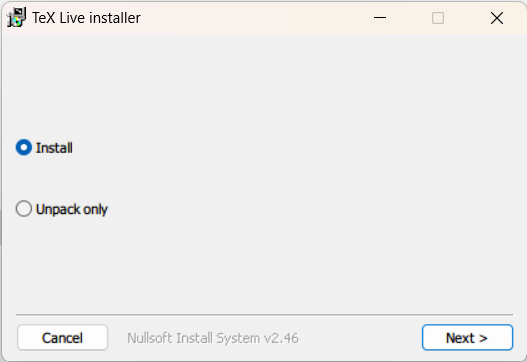
\includegraphics[width=\linewidth]{src/install_windows_1.png}
    \caption{インストールウィンドウ(Windows)(1)}
    \label{fig:ins_win_1}
  \end{minipage}%
  \hspace{.01\textwidth}
  \begin{minipage}[b]{.49\textwidth}
    \centering
    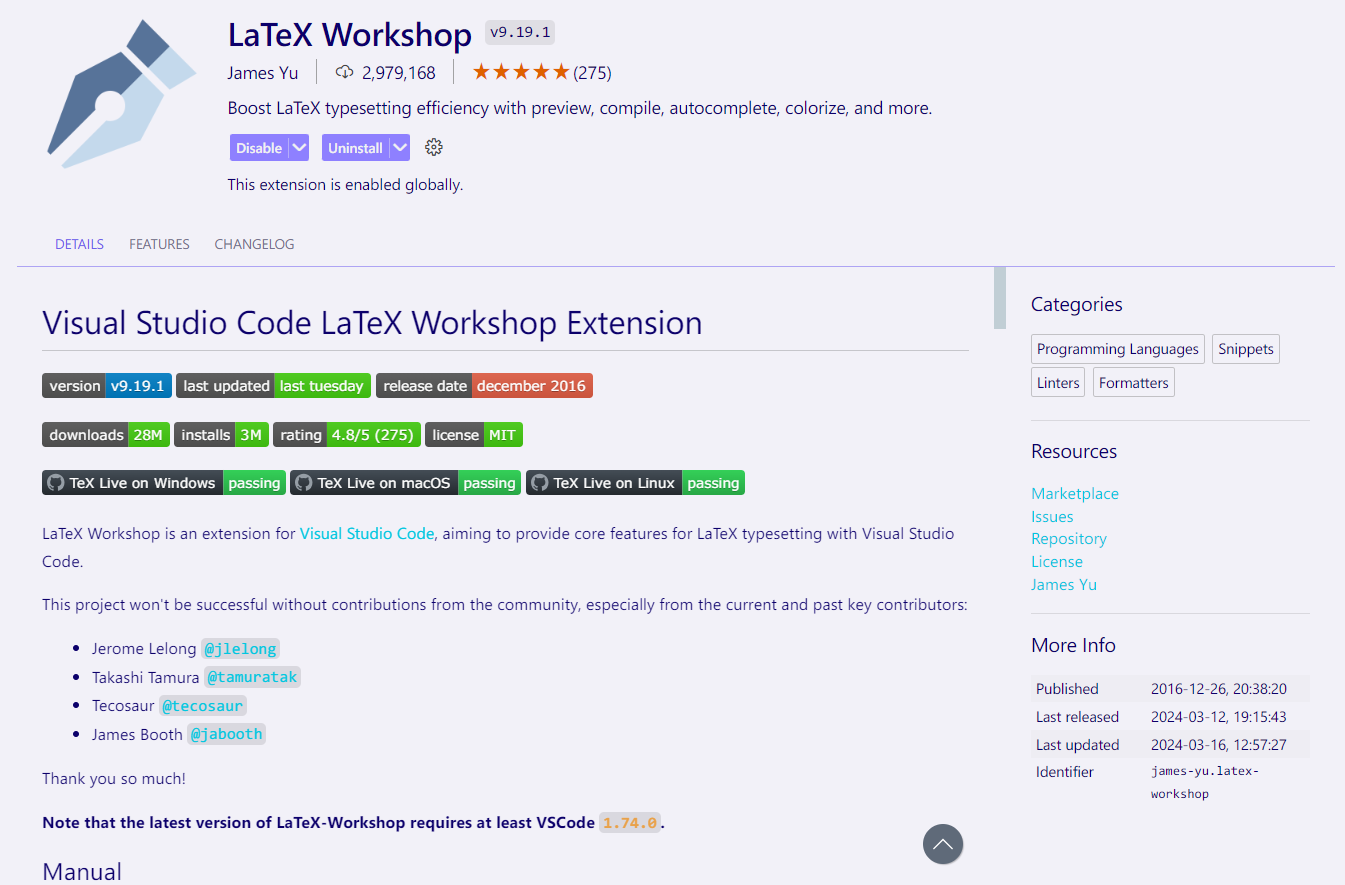
\includegraphics[width=\linewidth]{src/install_windows_2.png}
    \caption{LaTeX Workshop拡張機能}
    \label{fig:ins_win_2}
  \end{minipage}
\end{figure}

\subsubsection{Linux (Ubuntu)の場合}
Linuxでは,流れとしてはWindowsでのインストール方法と大差は無いが,基本的に
コンソール上ですべての工程を行う.
まず,ミラーサイトから\texttt{instal-tl-unx.tar.gz}をダウンロードする必要があるので,
wgetまたはcurlコマンドを使用する.\\
wgetコマンドの場合は,\\
\texttt{wget http://mirror.ctan.org/systems/texlive/tlnet/install\\-tl-unx.tar.gz}\\
curlコマンドの場合は.\\
\texttt{curl -OL http://mirror.ctan.org/systems/texlive/tlnet/install-tl-unx.tar.gz}\\
このコマンドを実行したら,次はダウンロードしたインストーラのファイルを展開する.\\
\texttt{tar xvf install-unx.tar.gz}\\
展開したインストーラのディレクトリに移動する.\\
\texttt{cd install-tl-2*}\\
root権限でインストーラを実行する.\\
\texttt{sudo /install-tl -no-gui -repository \\
  http://mirror.ctan.org/systems/texlive/tlnet/}\\
この時,以下のような表示が出るので,Iを入力してインストールを開始する.
\texttt{
  Actions: \\
  <I> start  installation to hard disk\\
  <H> help\\
  <Q> quit\\
  \\
  Enter command:
}\\
インストールが終了したら/usr/local/binディレクトリは以下にシンボリックリンクを追加する.\\
\texttt{sudo /usr/local/texlive/????/bin/*/tlmgr path add}\\
途中の?や*はワイルドカード検索のため,自動的にうまく実行されるはずだが,そうでない場合は以下の
ように具体的なディレクトリ名を指定する.
\texttt{sudo /usr/local/texlive/2024/bin/x86\_64-linux/tlmgr path add}\\
もし以上の解説でうまくいかない場合は,TeXWikiのインストールガイド(\url{https://texwiki.texjp.org/?Linux})を参照してほしい.

\subsubsection{Mac OSの場合}
Mac OSでは,Mac向けのTeX LiveのパッケージであるMacTeXの導入が推奨されている.
基本的にはフルインストールを推奨するので,以下にフルインストールのためのコマンドを紹介する.
\begin{itemize}
  \item GUIアプリケーションありの場合\\
        \noindent
        \texttt{
          brew install --cask mactex\\
          sudo tlmgr update --self --all\\
          sudo tlmgr paper a4
        }
  \item GUIアプリケーションなしの場合\\
        \texttt{
          brew install --cask mactex-no-gui\\
          sudo tlmgr update --self --all\\
          sudo tlmgr paper a4
        }
\end{itemize}
Homebrewが入っていない場合はHomebrew公式HPからダウンロード・インストールすること.\\
Homebrew日本語公式ホームページ: \url{https://brew.sh/ja/}

\subsection{VS CodeにTeXの拡張機能を追加する}
TeX Liveのインストールが終われば, 次はVS Codeから\TeX をコンパイルできるようにする
必要がある. まず, \TeX の拡張機能をインストールしよう. VS Codeの「拡張機能」にて,
「LaTeX Workshop」と検索すれば同名の拡張機能が出てくるため, それをインストールする.
(図\ref{fig:ins_win_2}参照)\\

基本的には以上で作業は完了である.
% \section{\LaTeX の基本・テキスト編}
\subsection{パッケージ}
\subsubsection{パッケージとは・パッケージの使い方}
\LaTeX の最大の特徴はパッケージによって多彩な機能を追加できる点である.ではパッケージとはどういうものかというと,いくつかの機能をまとめて使えるようにした,いわばお道具箱のようなものである.例えば,テキストに色をつけたい時,\texttt{xcolor}パッケージを
読み込めばそれを使うことができる.どのように読み込めば良いかというと.\\
\texttt{
\indent
\textbackslash usepackage\{xcolor\}
}\\
とプリアンブルに書くことで読み込むことができる.
\subsection{章立て}
\subsubsection{章立ての方法}
レポートにおいて,章立ては必須である.章立てをする際には以下のタグを用いる.
\begin{itemize}
  \item \ttfamily \textbackslash section
  \item \textbackslash subsection
  \item \textbackslash subsubsection
  \item \textbackslash paragraph
\end{itemize}
\texttt{section}は行った実験ごとに章を分ける場合に使用し,\texttt{subsection}はその実験の各項目(目的,実験方法など)
を分けるのに使用する場合が多い.\texttt{subsubsection}に関しては更に細かく章を分けたいときに使用する.\texttt{paragraph}は,
更に細かい章分けに用いる.\\
例えば,工学部2年後期から始まる実験では,数日に分けて実験を行う場合が多いので,以下のように章立てをするのが良いだろう.
\begin{itembox}[c]{章立ての例}
  \ttfamily
  \textbackslash section\{1日目 実験内容\}\\
  \textbackslash subsection\{実験目的\}\\
  $\vdots$\\
  \textbackslash subsection\{考察\}\\
  \textbackslash section\{2日目 実験内容\}\\
  \textbackslash subsection\{実験目的\}\\
  $\vdots$
\end{itembox}
学部4年生以上は,所属する研究室や論文を提出する学会のルールに従うこと.
\subsection{文字の装飾}
論文やレポートなどを執筆したいとき,\textbf{太字}や\textit{Italic},\color{red}色付き文字\color{black}などを使って強調したいことがあるだろう.そこで\LaTeX で使える文字のスタイライズコマンドを以下に示す.
\subsubsection{太字}
太字を挿入したいときは,\texttt{textbf}コマンドを使用する.具体的には,次のように使う.
\begin{itembox}[c]{太字の例}
  \ttfamily
  \textbackslash textbf\{太字にしたい文\}
\end{itembox}
\subsubsection{Italic(斜体)}
斜体に関しては,日本語フォントに斜体が組み込まれていないため,基本的には日本語の斜体はサポートされていない.正確には全くできないというわけではないが,複雑かつ体裁が崩れやすいため,本誌では紹介しない.
英語に関してはシンプルな手法でできるため,以下に斜体にするためのコマンドを示す.
\begin{itembox}[c]{斜体の例}
  \ttfamily
  \textbackslash textit\{斜体にしたい英文\}
\end{itembox}
\subsubsection{等幅}
ソースコードを一部示すときなど,一時的に等幅フォントを使用したい場合は\texttt{texttt}コマンドを使用する.具体的には,次のように使う.
\begin{itembox}[c]{等幅の例}
  \ttfamily
  \textbackslash texttt\{等幅にしたい文\}
\end{itembox}
\subsubsection{色付き文字}
テキストの一部に色をつけたい場合は,\texttt{color}コマンドを使用する.なお,使用できる色については読み込むパッケージに依存しており,xcolorパッケージではさまざまな色が使える.逆にパッケージを読み込まなければ多彩な色付き文字を使うことはできないので,冒頭でxcolorパッケージを読み込まなければならない.
具体的には,次のように使う.
\begin{itembox}[c]{色付き文字の例}
  \ttfamily
  \textbackslash usepackage[dvipsnames]\{xcolor\}
  \% xcolorパッケージをdvipsnamesで読み込み(これで多彩な色を使える)
  \\
  中略
  \\
  \textbackslash color\{色\}色付きにしたい文\textbackslash color\{black\}
\end{itembox}
xcolorパッケージで使用できる色については,OverLeafのドキュメントを参考にすると良い.(\url{https://ja.overleaf.com/learn/latex/Using_colors_in_LaTeX})
% \section{さまざまな「環境」}
\subsection{「環境」とは}
図表を挿入する際,\LaTeX では「環境(environment)」というものを宣言し,その中に図表を挿入する.環境は挿入するものによって分けられており,以下のように対応している.
\begin{description}
  \item[箇条書き]: itemize環境(順番をつけるときはenumerateなど)
  \item[数式]: align環境,equation環境など
  \item[図]: figure環境
  \item[表]: table環境
\end{description}
他にも様々な環境が存在するが,本誌では代表的な環境を紹介する.
また,環境を使用するときは基本的に\texttt{begin}コマンドではじめ,\texttt{end}コマンドで終了する.例えば,itemize環境を用いるときは以下のようになる.
\begin{itembox}[c]{環境の使い方}
  \texttt{
    \hspace{-0.5\zw}\textbackslash begin\{itemize\}\\
    \hspace{2\zw}\textbackslash item アイテムA\\
    \hspace{2\zw}\textbackslash item アイテムB\\
    \textbackslash end\{itemize\}
  }
\end{itembox}
\subsection{箇条書き}
通常の箇条書きにはitemizeを用いる.また,箇条書きする内容の先頭には\texttt{\textbackslash item}とつける必要がある.他にも箇条書きで用語を説明するdescriptionや,数字がつくenumerateも存在する.それぞれの例を以下に示していく.
\newpage
\subsubsection{itemizeの場合}
\begin{itembox}[c]{itemize環境を使う時のソースコード}
  \texttt{
    \hspace{-0.5\zw}\textbackslash begin\{itemize\}\\
    \hspace{2\zw}\textbackslash item アイテムA\\
    \hspace{2\zw}\textbackslash item アイテムB\\
    \textbackslash end\{itemize\}
  }
\end{itembox}
\begin{itemize}
  \item アイテムA
  \item アイテムB
\end{itemize}
\subsubsection{descriptionの場合}
\begin{itembox}[c]{description環境を使う時のソースコード}
  \texttt{
    \hspace{-0.5\zw}\textbackslash begin\{description\}\\
    \hspace{2\zw}\textbackslash item[説明A] アイテムA\\
    \hspace{2\zw}\textbackslash item[説明B] アイテムB\\
    \textbackslash end\{description\}
  }
\end{itembox}
\begin{description}
  \item[説明A] アイテムA
  \item[説明B] アイテムB
\end{description}
\subsubsection{enumerateの場合}
\begin{itembox}[c]{enumerate環境を使う時のソースコード}
  \texttt{
    \hspace{-0.5\zw}\textbackslash begin\{enumerate\}\\
    \hspace{2\zw}\textbackslash item アイテムA\\
    \hspace{2\zw}\textbackslash item アイテムB\\
    \textbackslash end\{enumerate\}
  }
\end{itembox}
\begin{enumerate}
  \item アイテムA
  \item アイテムB
\end{enumerate}
\subsection{数式}
一行で完結する数式,または複数行の数式に一つの式番号を振りたい場合は\texttt{equation}を,複数行の数式にそれぞれ連続した式番号を振りたい場合は\texttt{align}を用いる.なお,式番号を振りたくない場合は「*(アスタリスク)」をequationやalignの直後につける.
\subsubsection{equation}
\begin{itembox}[c]{equation}
  \texttt{
    \hspace{-0.5\zw}\textbackslash begin\{equation\}\\
    \hspace{2\zw}e\textasciicircum\{i\textbackslash pi\}=-1\\
    \textbackslash end\{equation\}\\
    \textbackslash begin\{equation\}\\
    \hspace{2\zw}\textbackslash begin\{split\}\\
    \hspace{4\zw}\textbackslash cos\textasciicircum2\textbackslash theta \& = \textbackslash cos\textasciicircum2\textbackslash theta -\textbackslash sin\textasciicircum2\textbackslash theta \textbackslash \textbackslash\\
    \hspace{4\zw}\& = 2\textbackslash cos\textasciicircum2\textbackslash theta - 1          \textbackslash \textbackslash\\
    \hspace{4\zw}\& = 1 - 2\textbackslash sin\textasciicircum2\textbackslash theta\\
    \hspace{2\zw}\textbackslash end\{split\}\\
    \textbackslash end\{equation\}
  }
\end{itembox}
\begin{equation}
  e^{i\pi}=-1
\end{equation}
\begin{equation}
  \begin{split}
    \cos 2\theta & = \cos^2\theta -\sin^2\theta \\
                 & = 2\cos^2\theta - 1          \\
                 & = 1 - 2\sin^2\theta
  \end{split}
\end{equation}
\subsubsection{align}
\begin{itembox}[c]{align}
  \texttt{
    \hspace{-0.5\zw}\textbackslash begin\{align\}\\
    \hspace{4\zw}\textbackslash cos\textasciicircum2\textbackslash theta \& = \textbackslash cos\textasciicircum2\textbackslash theta -\textbackslash sin\textasciicircum2\textbackslash theta \textbackslash \textbackslash\\
    \hspace{4\zw}\& = 2\textbackslash cos\textasciicircum2\textbackslash theta - 1          \textbackslash \textbackslash\\
    \hspace{4\zw}\& = 1 - 2\textbackslash sin\textasciicircum2\textbackslash theta\\
    \textbackslash end\{align\}
  }
\end{itembox}
\begin{align}
  \cos 2\theta & = \cos^2\theta -\sin^2\theta \\
               & = 2\cos^2\theta - 1          \\
               & = 1 - 2\sin^2\theta
\end{align}

\subsection{図}
図を挿入する際にはfigure環境を用いる.figure環境を用いることで,図にキャプションをつけることができる.また,図の位置を指定することもできる.
\begin{itembox}[c]{figure環境を使う時のソースコード}
  \texttt{
  \hspace{-0.5\zw}\textbackslash begin\{figure\}[htbp]\\
  \hspace{4\zw}\textbackslash centering\\
  \hspace{4\zw}\textbackslash includegraphics[width=12cm]\{sample.jpg\}\\
  \hspace{4\zw}\textbackslash caption\{画像サンプル\}\\
  \textbackslash end\{figure\}
  }
\end{itembox}
\begin{figure}[htbp]
  \centering
  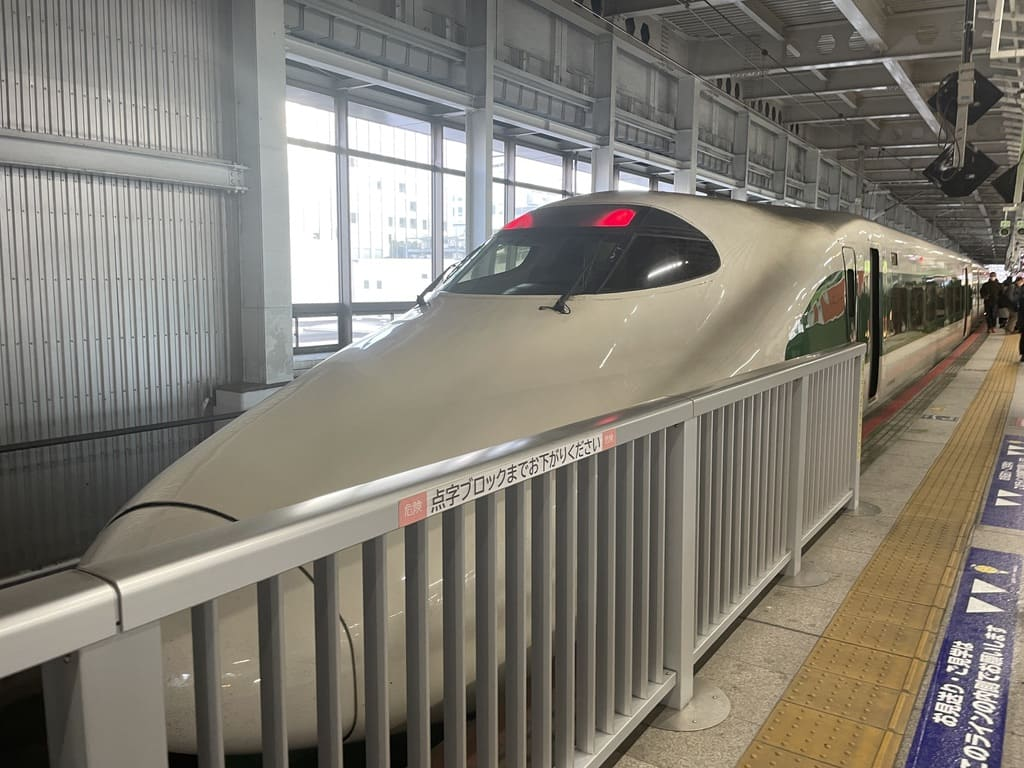
\includegraphics[width=12cm]{src/sample.jpg}
  \caption{画像サンプル}
\end{figure}
\subsection{表}
表を挿入する際にはtable環境を用いる.table環境を用いることで,表にキャプションをつけることができる.また,表の位置を指定することもできる.
\begin{itembox}[c]{table環境を使う時のソースコード}
  \texttt{
  \hspace{-0.5\zw}\textbackslash begin\{table\}[htbp]\\
  \hspace{4\zw}\textbackslash centering\\
  \hspace{4\zw}\textbackslash caption\{表サンプル\}\\
  \hspace{4\zw}\textbackslash begin\{tabular\}\{c|c\}\\
  \hspace{6\zw}\textbackslash hline タイトルA \& タイトルB \textbackslash\textbackslash\\
  \hspace{6\zw}\textbackslash hline 内容C \& 内容D \textbackslash\textbackslash\\
  \hspace{6\zw}\textbackslash hline 内容E \& 内容F \textbackslash\textbackslash\\
  \hspace{6\zw}\textbackslash hline\\
  \hspace{4\zw}\textbackslash end\{tabular\}\\
  \textbackslash end\{table\}
  }
\end{itembox}
\begin{table}[htbp]
  \centering
  \caption{表サンプル}
  \begin{tabular}{c|c}
    \hline
    タイトルA & タイトルB \\
    \hline
    内容C   & 内容D   \\
    \hline
    内容E   & 内容F   \\
    \hline
  \end{tabular}
\end{table}
\subsection{htbpとは}
図や表の位置を指定する際に,htbpというオプションを指定することがある.htbpはそれぞれ以下のような意味を持つ.
\begin{description}
  \item[h]: その場所に挿入
  \item[t]: ページの上部に挿入
  \item[b]: ページの下部に挿入
  \item[p]: 1ページにまとめて挿入
\end{description}
何も指定しない場合は,\LaTeX が自動で最適な位置に挿入する.しかし,ページ数が一番
少なくなるような位置に挿入するため,図や表が思った位置に挿入されないことが多い.
また,htbp指定でも必ずしも思った位置に挿入されるわけではない.どうしても図や表を
特定の位置に挿入したい場合は,hereパッケージを使って\texttt{[H]}オプションを
指定することで,その場所に図表を挿入できる.
% \section{参考文献の挿入}
参考文献を挿入するときはBibTeXを用いるのが便利である.BibTeXを用いると,文献情報を記述したファイル(.bib)を作成し,それを参照することで,文献リストを自動で生成することができる.
\subsection{BibTeXの使い方}
BibTeXを用いるためには,以下の手順を踏む必要がある.
\begin{enumerate}
  \item 参考文献情報を記述したファイル(.bib)を作成する
  \item \LaTeX ファイル内でBibTeXを読み込む
  \item 参考文献リストを挿入する
\end{enumerate}
\subsubsection{参考文献情報の記述}
参考文献情報を記述したファイル(.bib)は,以下のような形式で記述する.

% \section{体裁の調整}
\subsection{ページレイアウト}
余白を調整する方法には,いくつかの方法がある.
ここでは,geometryパッケージを用いた方法とパッケージを用いない方法を紹介する.
\subsubsection{geometryパッケージを用いた方法}
geometryパッケージを用いると,簡単にページレイアウトを調整することができる.
geometryパッケージを用いると,以下のように記述することで,ページレイアウトを調整することができる.
\begin{lstlisting}
\usepackage{geometry}
\geometry{left=3cm,right=3cm,top=3cm,bottom=3cm}
\end{lstlisting}
この場合,左右上下の余白をそれぞれ3cmに設定している.
また,このように指定する方法もある.
\begin{lstlisting}
\usepackage[top=3cm,bottom=3cm,left=3cm,right=3cm]{geometry}
\end{lstlisting}
\subsubsection{パッケージを用いない方法}
パッケージを用いない方法でページレイアウトを調整する場合は,以下のように記述する.
\begin{lstlisting}
% 余白の設定 ---
\setlength{\textheight}{\paperheight}
\setlength{\topmargin}{4.6truemm}  % 上の余白を30mm (=1inch[25.4mm] - 4.6mm)に
\addtolength{\topmargin}{-\headheight}
\addtolength{\topmargin}{-\headsep}
\addtolength{\textheight}{-60truemm} % 下の余白も30mmに (TOP+20mm)

\setlength{\textwidth}{\paperwidth}
\setlength{\oddsidemargin}{4.6truemm}  % 左の余白を30mm (=1inch[25.4mm] + 4.6mm)に
\setlength{\evensidemargin}{\oddsidemargin}
\addtolength{\textwidth}{-61truemm} % 右の余白も30mmに
% ---
\end{lstlisting}
ちなみにこれは本書の設定である.
また,インデントなどの幅を細く変えたいとき,単位を用いる時がある.
このとき,単位として使用できるのは以下の通りである.
\begin{itemize}
  \item mm - ミリメートル.1mmは1ミリメートルに相当する単位. 
  \item cm - センチメートル.1cmは10ミリメートルに相当する単位.
  \item in - インチ.1inは2.54cm(25.4mm)に相当する単位.
  \item pt - ポイント.1ptは1/72インチ(約0.3527mm)に相当する単位.
  \item em - em単位.その場で使われているフォントサイズ(ポイント数)に相当する相対単位.例えば、12ptのフォントなら1emは12pt. 
  \item ex - ex単位.フォントのx高さに基づく相対単位で、x文字の高さを基準とする.フォントによって変動する. 
  \item mu - mu単位.1muは1/18emに相当する非常に小さな単位で、主に数式内の余白調整に使用される. 
  \item zh - 全角文字の高さに基づく単位.CJK(中国語,日本語,韓国語)用の文字サイズに対応. 
  \item zw - 全角文字の幅に基づく単位.
  \item \% - パーセンテージ.例えば,ページやカラムの幅の何\% かを指定する際に使用する.
  \item \textbackslash linewidth - 現在の段落の幅を指定する.段落内での相対的な長さ調整に使える. 
  \item \textbackslash textheight - 本文領域の高さを指定する.ページ内の文章領域のサイズ調整に使われる. 
  \item \textbackslash paperheight - 紙全体の高さを指定する.文書全体のレイアウト設計に使用する. 
  \item \textbackslash paperwidth - 紙全体の幅を指定する.文書全体のレイアウト設計に使用する. 
  \item \textbackslash textwidth - 本文領域の幅を指定する.文章の横幅を設定するための重要な単位. 
  \item \textbackslash columnwidth - カラムの幅を指定する.2カラムや複数カラムのレイアウトで使われる. 
  \item \textbackslash columnsep - カラム間の間隔を指定する.カラム間の余白の調整に使用される. 
  \item \textbackslash columnseprule - カラム間のルールの幅を指定する.カラム間の罫線の太さを調整できる.
\end{itemize}
\subsection{ページスタイル}
fancyhdrパッケージを用いると,ページスタイルを少し変えることができる.
以下のように記述することで,ページスタイルを変更することができる.
\begin{lstlisting}
% ページスタイルの設定 ---
\pagestyle{fancy}
\lhead{}
\chead{}
\rhead{}
\lfoot{}
\cfoot{--\;\thepage\;--}
\rfoot{}
\end{lstlisting}
この場合,ページの中央下部にページ番号が表示される.
本書では,各章で右上に章番号と章名,中央下にページ番号を表示するように設定している.
\subsection{段組}
multicolパッケージを用いると,段組を簡単に設定することができる.
以下のように記述することで,段組を設定することができる.
\begin{lstlisting}
\usepackage{multicol}
\begin{multicols}{2}
  ここに段組したい文章を記述する.
\end{multicols}
\end{lstlisting}
この場合,2つの段組を設定している.
他には,documentclassのオプションでtwocolumnを指定することで,2段組にすることもできる.
% \bibliography{resume}
% \bibliographystyle{junsrt}
\end{document}
